% !TeX root = RJwrapper.tex
%\title{ClusROC: An R package for ROC analysis in three-class classification problems for clustered data}
\title{ClusROC: An R Package for ROC Analysis in Three-Class Classification Problems for Clustered Data}
\author{by Duc-Khanh To, Gianfranco Adimari, and Monica Chiogna}

\maketitle

\abstract{%
This paper introduces an R package for ROC analysis in three-class classification problems, for clustered data in the presence of covariates, named ClusROC. The clustered data that we address have some hierarchical structure, i.e., dependent data deriving, for example, from longitudinal studies or repeated measurements. This package implements point and interval covariate-specific estimation of the true class fractions at a fixed pair of thresholds, the ROC surface, the volume under the ROC surface, and the optimal pairs of thresholds. We illustrate the usage of the implemented functions through two practical examples from different fields of research. 
}

\hypertarget{introduction}{%
\section{Introduction}\label{introduction}}

In clinical studies, receiver operating characteristic (ROC) surface analysis is widely used to evaluate the accuracy of a diagnostic test (or biomarker) when there are three ordinal disease classes (or diagnostic groups). See \citet{nak:14} for a comprehensive review. Although the clinical context is where ROC surface analysis finds its natural application, other contexts,  such as economics and engineering, very often face the problem of evaluating the accuracy of a classifier.

Within the ROC surface analysis framework, the following quantities are typically objects of interest: ROC surface, VUS (volume under ROC surface), and optimal pair of thresholds. Statistical methods for evaluating such quantities have been widely discussed in the statistical literature. We cite, among others, papers by \citet{nak:04}; \citet{xiong2006measuring}; \citet{nakas2010accuracy}; \citet{attwood2014diagnostic}; \citet{bantis2017construction}; \citet{toduc2016mar}. Moreover, on the Comprehensive R Archive Network (CRAN), there are several packages implementing estimation methods for ROC surface analysis, for instance, \CRANpkg{trinROC} \citep{trinROC}, \CRANpkg{ThresholdROC} \citep{ThresholdROC} and \CRANpkg{bcROCsurface} \citep{bcROCsurface}.

Most of the existing methods for ROC surface analysis have focused on a standard setting, in which measurements on statistical units are realizations of independent random variables, and the diagnostic test, or, more broadly, the classifier, is not influenced by any covariate. In some studies, however, not only the classifier can be affected by some covariates that characterize the units themselves (e.g.~age, gender), but statistical units can be enrolled in clusters (e.g., families, genotype, communities, etc.). When statistical units are drawn from clusters, they can no longer be treated as independent. Indeed, units from the same cluster are typically more similar to each other than they will be to statistical units from other clusters. Therefore, unobserved variables may induce statistical dependence between observations within clusters that may be uncaptured by covariates. For such kinds of clustered data, which have a hierarchical structure and are dependent, \citet{xiong2018estimating} proposed the use of a standard linear {mixed-effects} model \citep{mcculloch2004generalized} to account for clusters and covariates' effects on the {classifier}. Then, the authors developed an approach to estimate the VUS, under an assumption of normality. Based on the model in \citet{xiong2018estimating}, \citet{khanh2022} developed an estimation procedure for the ROC surface and methods for choosing the optimal pair of thresholds. The authors also discussed a variant of their approach, based on the Box-Cox transformation, useful when the normality assumption is (not heavily) violated.

In this paper, we introduce our R package for ROC surface analysis with clustered data, named \CRANpkg{ClusROC}. The package (with related details) is available on CRAN at \url{http://CRAN.Rproject.org/package=ClusROC}. In the package, we implement procedures for estimating the parameters of the models (with and without the Box-Cox transformation), and for making inferences about the ROC surface, and the optimal pair of thresholds, by following methods outlined in \citet{khanh2022}. In addition, we also implement a procedure for estimating the VUS, as discussed in \citet{xiong2018estimating}.

In the following sections, we first briefly present the reference model and the inferential procedures for ROC surface analysis with clustered data. Then, we describe the \CRANpkg{ClusROC} package and illustrate its use through two real datasets. The last section provides a brief conclusion.

\hypertarget{roc-surface-analysis-for-clustered-data}{%
\section{The ROC surface analysis for clustered data}\label{roc-surface-analysis-for-clustered-data}}

Here we briefly review methods proposed by \citet{xiong2018estimating} and \citet{khanh2022}. Details and theoretical results can be found in the original articles. {For convenience, as in the quoted papers, we refer to some clinical studies in the presentation and use appropriate language for that area.}

\hypertarget{the-models}{%
\subsection{The models}\label{the-models}}

Let $Y$ be the diagnostic test result, on a continuous scale, and let $Y_1, Y_2, Y_3$ be the test results for subjects in classes 1, 2, and 3, respectively. We assume that higher values of test results are associated with higher severity of the disease, and the severity of the disease grows with the class (i.e., class 3 is the worst). Let $X_1, \ldots, X_p$ be $p$ covariates, possibly associated with the test $Y$.

Let $c$ be the total number of clusters, randomly selected from the population. For the $k$-th cluster, $k=1, \ldots, c$, let $n_{ki}$ be the total number of subjects belonging to class $i$, $i = 1,2,3$ and let $n_k = n_{k1} + n_{k2} + n_{k3}$ be the total sample size within the cluster. Note that $n_{ki}$ might be equal to 0 for some clusters. The linear {mixed-effects} model for the clustering effect on the test result $Y$, as well as for covariates' effects, is written as follows \citep{xiong2018estimating, khanh2022}: 
\begin{eqnarray}
    Y_{1} &=& \alpha_{k_1} + z_1^\top \boldsymbol{\beta}_1 + \varepsilon_{1}, \nonumber \\
    Y_{2} &=& \alpha_{k_2} + z_2^\top  \boldsymbol{\beta}_2 + \varepsilon_{2}, \label{eq:modellmm} \\
    Y_{3} &=& \alpha_{k_3} + z_3^\top \boldsymbol{\beta}_3 + \varepsilon_{3}, \nonumber
\end{eqnarray}
where $(Y_1, Y_2, Y_3)$ is a triplet of test scores from three randomly sampled subjects from the three disease classes, $(k_1, k_2, k_3)$, $k_i \in \{1, \ldots, c\}$, are cluster memberships indicating the clusters from which $Y_1, Y_2, Y_3$ are observed, $z_i = (1, x_{1i}, \ldots, x_{pi})^\top$ are fixed (i.e., not random) covariates values, and $\boldsymbol{\beta}_i = (\beta_{0i}, \beta_{1i}, \ldots, \beta_{pi})^\top$, $i=1,2,3$, are vectors of parameters representing covariates effects. In model \eqref{eq:modellmm}, $\alpha_{k}$ are random effects accounting for the presence of clusters, and $\varepsilon_{i}$ are subject-level random errors. We assume that: (i) the random effects $\alpha_{k}$ and the subject-level random errors  $\varepsilon_{i}$ follow a normal distribution, i.e., $\alpha_{k} \sim \mathcal{N}(0, \sigma^2_c)$ and $\varepsilon_{i} \sim \mathcal{N}(0, \sigma^2_i)$ with $i = 1,2,3$; (ii) $\alpha_{1}, \alpha_{2}, \ldots, \alpha_{c}$ and $\varepsilon_{1}, \varepsilon_{2}, \varepsilon_{3}$ are all independent \citep[see also,][]{mcculloch2004generalized}.

Let $\boldsymbol{\beta} = (\boldsymbol{\beta}_1^\top, \boldsymbol{\beta}_2^\top, \boldsymbol{\beta}_3^\top)^\top$ with $\boldsymbol{\beta}_i = (\beta_{0i}, \beta_{1i}, \ldots, \beta_{pi})^\top$, and $\boldsymbol{\theta} = (\sigma_c, \sigma_1, \sigma_2, \sigma_3)^\top$ be the unknown parameters in model \eqref{eq:modellmm}. By using a restricted (or residual) maximum likelihood (REML) estimation approach, a consistent estimator $\widehat{\boldsymbol{\gamma}} = (\widehat{\boldsymbol{\beta}}^\top, \widehat{\boldsymbol{\theta}}^\top)^\top$ of $\boldsymbol{\gamma} = (\boldsymbol{\beta}^\top, \boldsymbol{\theta}^\top)^\top$ can be obtained. Under some regularity conditions, we have $\widehat{\boldsymbol{\gamma}} \stackrel{.}{\sim} \mathcal{N}(\boldsymbol{\gamma}, \boldsymbol{\Lambda})$. The asymptotic covariance matrix $\boldsymbol{\Lambda}$ can be consistently estimated by using the sandwich formula \citep{liang1986longitudinal, kauermann2001note, mancl2001covariance}.

In some practical situations, data distributions may be skewed and the {normality assumption} might be violated. For such cases, \citet{khanh2022} considered the application of Box-Cox transformation for linear {mixed-effects} models
\citep{lipsitz2000using, gurka2006extending}: 
\begin{eqnarray}
    Y^{(\lambda)}_{1} &=& \alpha_{k_1} + z_1^\top \boldsymbol{\beta}_1 + \varepsilon_{1}, \nonumber \\
    Y^{(\lambda)}_{2} &=& \alpha_{k_2} + z_2^\top \boldsymbol{\beta}_2 + \varepsilon_{2}, \label{eq:modellmmbxc} \\
    Y^{(\lambda)}_{3} &=& \alpha_{k_3} + z_3^\top \boldsymbol{\beta}_3 + \varepsilon_{3}, \nonumber
\end{eqnarray} 
where $Y^{(\lambda)}_{i}$ is the Box-Cox transformed response, $Y^{(\lambda)}_{i} = (Y^{\lambda}_{i} - 1)/\lambda$ if $\lambda \ne 0$ and $Y^{(\lambda)}_{i} = \log(Y_{i})$ if $\lambda = 0$, with $i = 1,2,3$, $Y_{i} > 0$, and $\lambda$ is the transformation parameter \citep{box1964analysis}. Assumptions about the random effects $\alpha_{k}$ and the subject-level random errors $\varepsilon_{i}$ are the same as in model \eqref{eq:modellmm}. To obtain $\widehat{\lambda}$ and the REML estimator $\widehat{\boldsymbol{\gamma}}$, \citet{khanh2022} applied the method proposed by \citet{gurka2011estimating} which is based on the scaled Box-Cox transformation model \citep{gurka2006extending}. The estimator of the variance-covariance matrix of the REML estimator $\widehat{\boldsymbol{\gamma}}$ is obtained again by applying the sandwich formula.

\hypertarget{roc-surface-analysis}{%
\subsection{ROC surface analysis}\label{roc-surface-analysis}}

According to the model \eqref{eq:modellmm}, at a given vector $z$ of covariates' values, $Y_i \sim \mathcal{N}(z^\top \boldsymbol{\beta}_i, \sigma^2_c + \sigma^2_i)$ with $z = (1, x_{1}, \ldots, x_{p})^\top$ and $i = 1, 2, 3$. \citet{khanh2022} further assume that $z^\top \boldsymbol{\beta}_1 < z^\top \boldsymbol{\beta}_2 < z^\top \boldsymbol{\beta}_3$, i.e., that the stochastic dominance for the three classes holds at $z$.

For given thresholds $t_1$ and $t_2$ ($t_1 < t_2$), the covariate-specific true class fractions (TCFs) are written as $\mathrm{TCF}_1(t_1;z) = \Phi\left(\frac{t_1 - z^\top \boldsymbol{\beta}_1}{\sqrt{\sigma^2_c + \sigma^2_1}}\right)$, $\mathrm{TCF}_2(t_1, t_2;z) = \Phi\left(\frac{t_2 - z^\top \boldsymbol{\beta}_2}{\sqrt{\sigma^2_c + \sigma^2_2}}\right) - \Phi\left(\frac{t_1 - z^\top \boldsymbol{\beta}_2}{\sqrt{\sigma^2_c + \sigma^2_2}}\right)$ and $\mathrm{TCF}_3(t_2;z) = 1 - \Phi\left(\frac{t_2 - z^\top \boldsymbol{\beta}_3}{\sqrt{\sigma^2_c + \sigma^2_3}}\right)$, where $\Phi(\cdot)$ is the cumulative distribution function of the standard normal distribution. Moreover, by setting $\mathrm{TCF}_1(t_1;z) = p_1$ and $\mathrm{TCF}_3(t_2;z) = p_3$, the covariate-specific ROC surface can be defined as a function of $(p_1, p_3)$, i.e., 
\begin{eqnarray}
\mathrm{ROCs}(p_1, p_3; z) &=& \Phi\left(\frac{\Phi^{-1}(1 - p_3)\sqrt{\sigma^2_c + \sigma^2_3} + z^\top \boldsymbol{\beta}_3 - z^\top \boldsymbol{\beta}_2}{\sqrt{\sigma^2_c + \sigma^2_2}}\right) \nonumber \\
&& - \: \Phi\left(\frac{\Phi^{-1}(p_1)\sqrt{\sigma^2_c + \sigma^2_1} + z^\top \boldsymbol{\beta}_1 - z^\top \boldsymbol{\beta}_2}{\sqrt{\sigma^2_c + \sigma^2_2}}\right), \label{eq:rocs}
\end{eqnarray}
if
$\Phi^{-1}(p_1) < \frac{\Phi^{-1}(1 - p_3)\sqrt{\sigma^2_c + \sigma^2_3} + z^\top \boldsymbol{\beta}_3 - z^\top \boldsymbol{\beta}_1}{\sqrt{\sigma^2_c + \sigma^2_1}}$; otherwise, $\mathrm{ROCs}(p_1, p_3; z) = 0$.

Based on the above expressions, for clustered data, \citet{khanh2022} considered covariate-specific estimation of the TCFs at a fixed pair of thresholds $(t_1, t_2)$ and estimation of the ROC surface for each pair $(p_1, p_3)$. Moreover, the authors proposed methods to estimate covariate-specific optimal pairs of thresholds $(t_1^+, t_2^+)$ by considering three different criteria: (i) maximization of the covariate-specific generalized Youden index (GYI); (ii) minimization of the covariate-specific Euclidean distance between the ideal point $(1, 1, 1)$ and the point $\left(\mathrm{TCF}_1(t_1;z), \mathrm{TCF}_2(t_1, t_2;z), \mathrm{TCF}_3(t_2;z)\right)$ (CtP); (iii) maximization of the covariate-specific volume of the cuboid under the covariate-specific ROC surface (MV). Resulting estimators are shown to be consistent and asymptotically normal, with asymptotic covariance matrices estimable by using the plug-in method. The normal approximation results can be used to construct suitable (joint) confidence regions.

Starting from model \eqref{eq:modellmm}, covariate-specific inference on the VUS is discussed in \citet{xiong2018estimating}, where maximum likelihood (ML) methods for point and interval estimation are proposed. In particular, \citet{xiong2018estimating} showed that covariate-specific ML VUS estimator $\hat{\theta}(z)$ is the summation of five components: $\hat{\theta}_1(z) = \widehat{\Pr}(Y_1 < Y_2 < Y_3, k_1 = k_2 = k_3|z)$, $\hat{\theta}_2(z) = \widehat{\Pr}(Y_1 < Y_2 < Y_3, k_1 = k_2 \ne k_3|z)$, $\hat{\theta}_3(z) = \widehat{\Pr}(Y_1 < Y_2 < Y_3, k_1 = k_3 \ne k_2|z)$, $\hat{\theta}_4(z) = \widehat{\Pr}(Y_1 < Y_2 < Y_3, k_1 \ne k_2 = k_3|z)$, and $\hat{\theta}_5(z) = \widehat{\Pr}(Y_1 < Y_2 < Y_3, k_1 \ne k_2 \ne k_3|z)$.

In cases where the assumption of normality for $Y_1$, $Y_2$ and $Y_3$ is unrealistic, inferential procedures for covariate-specific TCFs, ROC surface, optimal pair of thresholds (and VUS) can be obtained starting from model \eqref{eq:modellmmbxc}; see Section 3.3 in \citet{khanh2022}.

\hypertarget{overview-of-r-package-clusroc}{%
\section{Overview of R package
ClusROC}\label{overview-of-r-package-clusroc}}

The \textbf{ClusROC} package implements techniques for ROC surface analysis, in case of clustered data and the presence of covariates. The package comprises five major functions:
{
\begin{itemize}
\item \texttt{clus\_lme()}: This function fits the linear mixed-effects model \eqref{eq:modellmm} under the normality assumption, or the model \eqref{eq:modellmmbxc} when the Box-Cox transformation is used.
\item \texttt{clus\_roc\_surface()}: This function estimates and makes a 3D plot of covariate-specific ROC surfaces.
\item \texttt{clus\_opt\_thres3()}: This function estimates the covariate-specific optimal pair of thresholds.
\item \texttt{clus\_vus()}: This function estimates the covariate-specific VUS.
\item \texttt{clus\_tcfs()}: This function estimates the covariate-specific TFCs at a specified pair of thresholds.
\end{itemize}
}

The \textbf{ClusROC} package can be installed directly from CRAN by using the code below:

\begin{example}
  install.packages("ClusROC")
\end{example}
Also, it can be installed from GitHub (``toduckhanh/ClusROC''), by using
the function \texttt{install\_github()} from \CRANpkg{devtools} package:


\begin{example}
  library(devtools)
  install_github("toduckhanh/ClusROC")
\end{example}


\hypertarget{description}{%
\subsection{Description}\label{description}}

The REML estimation in function {\texttt{clus\_lme()}} is based on the function \texttt{lme()} of package \CRANpkg{nlme} \citep{nlme}. The function {\texttt{clus\_lme()}} needs, firstly, specification of a {\texttt{fixed\_formula}} which is a two-sided linear formula object describing the fixed-effects part of the model for three classes, with the response on the left of \texttt{\textasciitilde{}} operator and the terms, separated by \texttt{+} operators, on the right. Secondly, the arguments {\texttt{name\_class}} and {\texttt{name\_clust}} are needed to specify the name of the variables indicating the disease classes (or diagnostic groups) and the clusters in the data, respectively. To enable the Box-Cox transformation, users need to set the argument \texttt{boxcox} as \texttt{TRUE}. The Box-Cox parameter $\lambda$ is estimated by a grid search on the interval $(-2, 2)$. This interval is suggested by \citet{gurka2011estimating}, but users can change this range by setting the argument \texttt{interval\_lambda}. Before fitting the model, {\texttt{clus\_lme()}} determines the ordering of the disease groups based on the average values of test results in each disease group. If an ordering is provided by the user via the argument {\texttt{levl\_class}}, the ordering of the mean values is still obtained to confirm the input ordering. In case of disagreement between the two orderings, the one based on the averages of test results is adopted. The function \texttt{plot()} provides three diagnostic plots for the model fitted by {\texttt{clus\_lme()}}, namely, a Q-Q plot for residuals, a Fitted vs. Residuals plot, and a Q-Q plot for cluster effects. These plots exploit the \CRANpkg{ggplot2} package \citep{ggplot2}.

The functions {\texttt{clus\_roc\_surface()}}, {\texttt{clus\_opt\_thres3()}}, {\texttt{clus\_vus()}} and {\texttt{clus\_tcfs()}} are the main functions to perform the ROC surface analysis for clustered data. All of them require the output of {\texttt{clus\_lme()}} as an argument. When one of the above functions is called, a check on the monotone ordering assumption is performed. That is, for a given value of the covariates, say $z$, the three predicted mean values of the test results in the three diagnostic groups, i.e., $z^\top \widehat{\boldsymbol{\beta}}_1$, $z^\top \widehat{\boldsymbol{\beta}}_2$ and $z^\top \widehat{\boldsymbol{\beta}}_3,$ are computed and compared. If the assumption ($z^\top \widehat{\boldsymbol{\beta}}_1 < z^\top \widehat{\boldsymbol{\beta}}_2 < z^\top \widehat{\boldsymbol{\beta}}_3$) is not met, the ROC surface analysis is not performed at $z$.

The function {\texttt{clus\_roc\_surface()}} estimates a covariate-specific ROC surface at a single point for covariates and makes a 3D plot to display the estimated covariate-specific ROC surface by using \CRANpkg{rgl} package \citep{rgl}. This function also allows plotting an ellipsoidal confidence region for TCFs at a given pair of thresholds, in the ROC surface space. If the constructed confidence region is outside the unit cube, a probit transformation \citep{bantis2017construction} is automatically applied to obtain an appropriate confidence region, which is inside the unit cube.

The function {\texttt{clus\_opt\_thres3()}} gives the estimated covariate-specific optimal pair of thresholds as defined by the criteria GYI, CtP, and MV at multiple points of the covariates. The optimization is done by using the function \texttt{optim()} with the ``L-BFGS-B'' method; however, users can select other optimization methods, such as, ``BFGS'' or ``Nelder-Mead''. The function returns also the estimated asymptotic variance-covariance matrix of the (estimated) covariate-specific optimal pair of thresholds. Under the {normality assumption}, the asymptotic variance-covariance matrix is estimated by the Delta method. If the Box-Cox transformation is applied, a nonparametric bootstrap procedure for clustered data is used to estimate the asymptotic variance-covariance matrix. To speed up the bootstrap procedure, users can set the argument \texttt{parallel} as \texttt{TRUE} to enable parallel computing support. Users can also select the number of CPUs needed for the computation. After calling {\texttt{clus\_opt\_thres3()}}, the function \texttt{plot()} can be used to display confidence regions (and point estimates) of covariate-specific optimal pairs of thresholds.

The function {\texttt{clus\_vus()}} estimates the covariate-specific VUS at multiple points of the covariates by using the \texttt{integrate()} routine. This function also performs the statistical test for the null hypothesis $H_0: VUS = 1/6$ versus the alternative $H_A: VUS > 1/6$. This statistical test is a formal assessment of the adequacy of a diagnostic test in a three-class classification problem via its VUS at given covariates values. After calling {\texttt{clus\_vus()}}, users can apply {\texttt{ci\_clus\_vus()}} to obtain confidence intervals for covariate-specific VUS. Three types of confidence intervals are computed: normal approximation-based; after logit and probit transformations.

The function {\texttt{clus\_tcfs()}} estimates covariate-specific TCFs at a specified pair of thresholds, given one or multiple points for the covariates. This function also implements the Delta method to estimate the asymptotic variance-covariance matrix of the estimated covariate-specific TCFs. Note that, if the Box-Cox transformation is applied for the linear {mixed-effects} model, the pair of threshold values must be provided in the original scale.

\hypertarget{applications}{%
\subsection{Applications}\label{applications}}

{To illustrate the use of the \textbf{ClusROC} package, we provide two examples with the \texttt{MouseNeurons} dataset and \texttt{EnergyEthiopia}, which are included in the package.}

\hypertarget{the-glutamatergic-neurons}{%
\subsubsection{The glutamatergic
neurons}\label{the-glutamatergic-neurons}}

\citet{khanh2022} used the \texttt{MouseNeurons} dataset to evaluate the ability of the Lysosomal Associated Membrane Protein Family Member 5 (Lamp5) gene to discriminate three types of glutamatergic neurons, namely Layer 2/3 Intratelencephalic (L2/3 IT), Layer 4 (L4) and Layer 5 Pyramidal Tract (L5 PT) neurons. A full version of the data is publicly available at \url{http://portal.brain-map.org/atlases-and-data/rnaseq/mouse-v1-and-alm-smart-seq}.

This dataset includes 860 observations (brain cells) and the following variables: the expression of the Lamp5 gene (diagnostic test/biomarker), the mouse genotype (which yields 23 clusters), the class labels (L2/3 IT, L4, and L5 PT), and the sex and age (in days) of the mouse. Below, we illustrate the use of the \textbf{ClusROC} package using this data.

\paragraph{Step 1: Load library and data}
\begin{example}
> library(ClusROC)
> data("MouseNeurons")
\end{example}
The above code loads the \textbf{ClusROC} package and the \texttt{MouseNeurons} data into \texttt{R}.

\paragraph{Step 2: Model fitting} \text{}\\
In this step, we fit a linear {mixed-effects} model with \texttt{Lamp5\_cpm} as a response and \texttt{age\_days} as a covariate, under the Box-Cox transformation, by using function \texttt{clus\_lme()}:

\begin{example}
> out_md <- clus_lme(fixed_formula = Lamp5_cpm ~ age_days, 
+                    name_class = "subclass_label", name_clust = "genotype_id", 
+                    data = MouseNeurons, boxcox = TRUE)
The ordered levels of classes are specified by the order of 
 averages of the test values for each class:
L4 < L5 PT < L2/3 IT 
\end{example}

\noindent
As, in this case, the rank-ordered nature of the biomarker concerning the classes is not given, the monotone ordering was specified by ordering the classes according to the rank of the biomarker's sample means in the three groups. The results are shown as follows.

\begin{example}
> print(out_md)

CALL: clus_lme(fixed_formula = Lamp5_cpm ~ age_days, name_class = "subclass_label", 
    name_clust = "genotype_id", data = MouseNeurons, boxcox = TRUE)
 
Coefficients:
                                   Est. Std.Error z-value p-value   
subclass_labelL4                0.78770   5.95328   0.132 0.89474   
subclass_labelL4:age_days       0.45039   0.18193   2.476 0.01330 * 
subclass_labelL5 PT            34.30543  12.27946   2.794 0.00521 **
subclass_labelL5 PT:age_days    0.20995   0.10652   1.971 0.04872 * 
subclass_labelL2/3 IT          49.34642  20.88162   2.363 0.01812 * 
subclass_labelL2/3 IT:age_days  0.08991   0.08306   1.082 0.27907   
sigma_c                         6.78582   4.15973      --      --   
sigma_1                        15.02492   7.12012      --      --   
sigma_2                        11.24066   5.70949      --      --   
sigma_3                        11.14321   6.07808      --      --
lambda                          0.44565        --      --      --   
ICC                             0.22848        --      --      --   
---
Signif. codes:  0 ‘***’ 0.001 ‘**’ 0.01 ‘*’ 0.05 ‘.’ 0.1 ‘ ’ 1

Number of observations: 860
Number of clusters: 23
Sample size within cluster:
     Min      Max  Average 
  1.0000 330.0000  37.3913 
Box-Cox transformation: TRUE
\end{example}

\noindent
The diagnostic plots for the fitted model are obtained by the following command (see Figure \ref{fig:diag-md}):

\begin{example}
> plot(out_md)
\end{example}

\begin{figure}[htbp]
\centering 
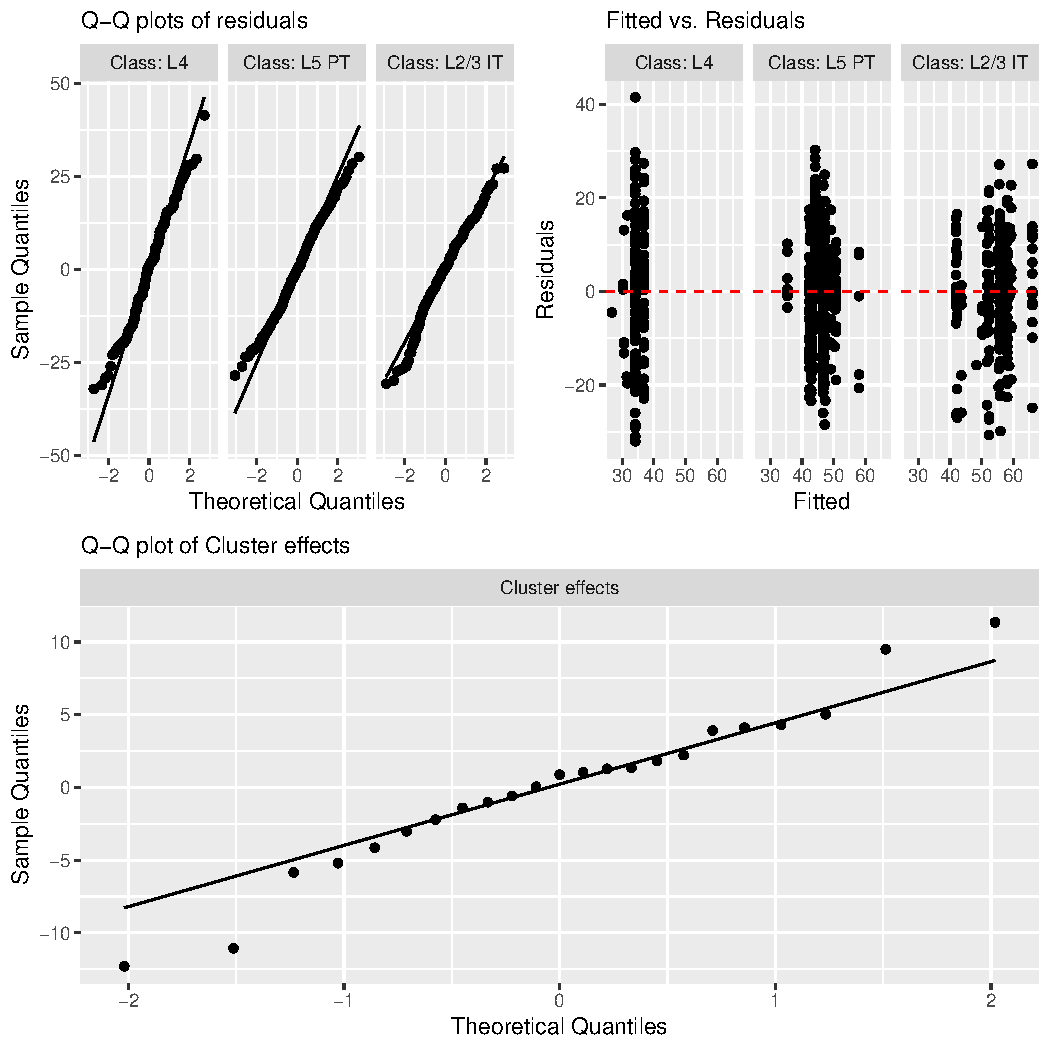
\includegraphics[width=0.7\linewidth]{diagnosis_model.pdf}
\caption{The diagnostic plots for the linear {mixed-effects} model.}
\label{fig:diag-md}
\end{figure}

\noindent
The plots suggest that the assumptions of normality and homogeneity of variances are satisfied. To help the reader evaluate the need for transforming the data, we also fitted the linear mixed-effects model without the Box-Cox transformation. The results are reported in Appendix, showing that the assumptions are violated.

\paragraph{Step 3: ROC surface analysis} \text{}\\
After fitting the linear {mixed-effects} models of interest and verifying the {normality assumption} and {the homogeneity of variances assumption}, the ROC surface analysis can be performed. First, let us start with the estimation for covariate-specific VUS.

\begin{example}
> out_vus <- clus_vus(out_clus_lme = out_md, 
+                     newdata = data.frame(age_days = c(54, 60, 66)))
> print(out_vus)

CALL: clus_vus(out_clus_lme = out_md, newdata = data.frame(age_days = c(54, 
    60, 66)))
 
Covariate-specific VUS: 
 Covariates Values  Est. Std.Error z-value p-value    
                54 0.541    0.0505    7.42  <0.001 ***
                60 0.514    0.0535    6.49  <0.001 ***
                66 0.485    0.0582    5.47  <0.001 ***
---
Signif. codes:    0 ‘***’ 0.001 ‘**’ 0.01 ‘*’ 0.05 ‘.’ 0.1 ‘ ’ 1
z-value and p-value are for testing the null hypothesis H0: VUS = 1/6 vs HA: VUS > 1/6 
\end{example}

\noindent
In this case, we are interested in computing the (estimated) covariate-specific VUS at three different ages of mice, i.e., 54, 60, and 66 days. The 95\% confidence intervals for covariate-specific VUS are obtained by:
{
\begin{example}
> ci_clus_vus(out_vus)

The 95% confidence intervals for covariate-specific VUS:
   Covariates Values  Normal approximation  Logit transformation  Probit transformation
                  54        (0.442, 0.640)        (0.442, 0.637)         (0.442, 0.638)
                  60        (0.409, 0.618)        (0.410, 0.616)         (0.410, 0.617)
                  66        (0.371, 0.599)        (0.374, 0.598)         (0.373, 0.599)
\end{example}
}
\noindent
As shown in the results, we can see three types of confidence intervals: normal approximation-based; after logit and probit transformations.

One obtains an estimate and a plot of the covariate-specific ROC surface, at, for example, the age of 58 days, as follows:
{
\begin{example}
> clus_roc_surface(out_clus_lme = out_md, newdata = data.frame(age_days = 58), 
+                  main = "Age-Specific ROC surface, at 58 days")
\end{example}
}
\noindent
The result is displayed in Figure \ref{fig:ROC-surface}(a). A plot of a 95\% ellipsoidal confidence region for TCFs at a fixed pair of threshold, for instance, $(t_1, t_2) = (350, 1350)$ is obtained as follows:
{
\begin{example}
> clus_roc_surface(out_clus_lme = out_md, newdata = data.frame(age_days = 58), 
+                  main = "Age-Specific ROC surface, at 58 days", 
+                  ellips = TRUE, thresholds = c(350, 1350))
\end{example}
}
\noindent
The 95\% ellipsoidal confidence region for TCFs and covariate-specific ROC surface are displayed in \ref{fig:ROC-surface}(b), together.
\begin{figure}[htbp]
\centering
\begin{tabular}{@{}c @{}c}
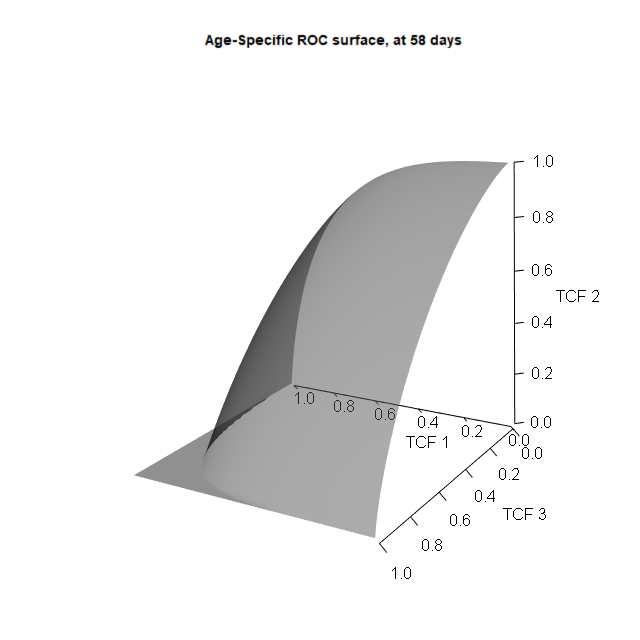
\includegraphics[width=0.5\textwidth]{ROCS_Age_58.png} & 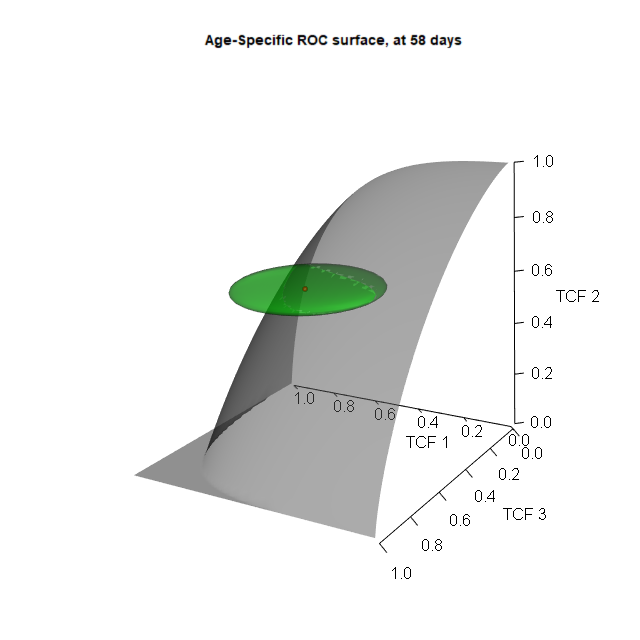
\includegraphics[width=0.5\textwidth]{ROCS_Age_58_ellip.png} \\
(a) & (b)
\end{tabular}
\caption{The plots of covariate-specific ROC surface at Age as 58 days: (a) without an ellipsoidal confidence region; (b) with an ellipsoidal confidence region for TCFs at $t_1 = 350$ and $t_2 = 1350$.}
\label{fig:ROC-surface}
\end{figure}

Estimates of covariate-specific TCFs at several values of the covariate, for a fixed pair of thresholds, are obtained by:
{
\begin{example}
> clus_tcfs(out_clus_lme = out_md, newdata = data.frame(age_days = c(54, 58, 62)), 
+           thresholds = c(350, 1350), ap_var = TRUE)

CALL: clus_tcfs(out_clus_lme = out_md, newdata = data.frame(age_days = c(54, 
    58, 62)), thresholds = c(350, 1350), apVar = TRUE)
 
Covariate-specific TCFs at (350,1350) : 
 Covariate(s) Values TCF 1 TCF 2 TCF 3 Se.TCF 1 Se.TCF 2 Se.TCF 3
                  54 0.576 0.632 0.522    0.113   0.0242   0.0630
                  58 0.533 0.620 0.533    0.119   0.0242   0.0604
                  62 0.490 0.607 0.544    0.124   0.0244   0.0592
\end{example}
}
\noindent
The results consist of three-point estimates of covariate-specific TCFs at the fixed pair of thresholds (350, 1350), corresponding to three different values of age, 54, 58, and 62 (days), and the associated standard errors (Se). Note that, for the function \texttt{roc\_surface()} and \texttt{clus\_tcfs()}, if the Box-Cox transformation is applied, the pair of thresholds values must be provided in the original scale.

The following call performs the estimation of the covariate-specific optimal pair of thresholds, and the corresponding asymptotic variance-covariance matrices, at three different ages of mice: 55, 65 and 75 days. Here, we consider all criteria, i.e., GYI, CtP and MV.

\begin{example}
> out_thresh <- clus_opt_thres3(method = c("GYI", "CtP", "MV"), out_clus_lme = out_md,
+                               newdata = data.frame(age_days = c(55, 65, 75)),
+                               ap_var = TRUE,
+                               control = list(n_boot = 1000, parallel = TRUE, 
+                                              ncpus = 8))
\end{example}

\noindent
In this case, a nonparametric bootstrap procedure for clustered data estimates the asymptotic variance-covariance matrix of the (estimated) covariate-specific optimal thresholds. Hence, we used a parallel computation with 8 CPUs ( Windows 10 Pro 64-bit, Intel(R) Core(TM) i7-7700, 3.6 GHz) to speed up this process ( the computation time for the parallel bootstrap process is about 15 minutes). As a general recommendation, we advise the user to switch to parallel computation not only in cases similar to the one tackled in this example but whenever the computational times appear to be too slow. The results are shown below.

\begin{example}
> print(out_thresh)

CALL: clus_opt_thres3(method = c("GYI", "CtP", "MV"), out_clus_lme = out_md, 
    newdata = data.frame(age_days = c(55, 65, 75)), ap_var = TRUE, 
    control = list(n_boot = 1000, parallel = TRUE, ncpus = 8))
 
Covariate-specific optimal pair of thresholds: 
 Covariate(s) Values                   Method Threshold 1 Threshold 2 TCF 1 TCF 2 TCF 3
                  55 Generalized Youden Index         530        1170 0.706 0.429 0.630
                  55    Closest to Perfection         446        1260 0.647 0.534 0.575
                  55               Max Volume         460        1260 0.658 0.525 0.575
                  65 Generalized Youden Index         627        1240 0.671 0.395 0.613
                  65    Closest to Perfection         538        1350 0.612 0.508 0.550
                  65               Max Volume         548        1350 0.619 0.502 0.550
                  75 Generalized Youden Index         731        1320 0.632 0.361 0.597
                  75    Closest to Perfection         639        1450 0.575 0.482 0.524
                  75               Max Volume         644        1450 0.578 0.480 0.523

Standard errors of Covariate-specific optimal pair of thresholds: 
 Covariate(s) Values                   Method SE. Threshold 1 SE. Threshold 2
                  55 Generalized Youden Index            61.1           130.0
                  55    Closest to Perfection            73.8            85.7
                  55               Max Volume            66.7            85.8
                  65 Generalized Youden Index            98.6           120.0
                  65    Closest to Perfection           115.0            87.1
                  65               Max Volume            98.7            84.3
                  75 Generalized Youden Index           133.0           147.0
                  75    Closest to Perfection           146.0           140.0
                  75               Max Volume           126.0           121.0
\end{example}

\noindent
The following call is needed to plot 95\% confidence regions for the covariate-specific optimal pairs of thresholds, and the result is shown in Figure \ref{fig:optThresh}.

\begin{example}
> plot(out_thresh, colors = c("forestgreen", "blue", "red"),
+      xlims = c(250, 1250), ylims = c(750, 1750), names.labels = "Age in days:",
+      size.point = 0.9)
\end{example}

\begin{figure}[htbp]
  \centering
  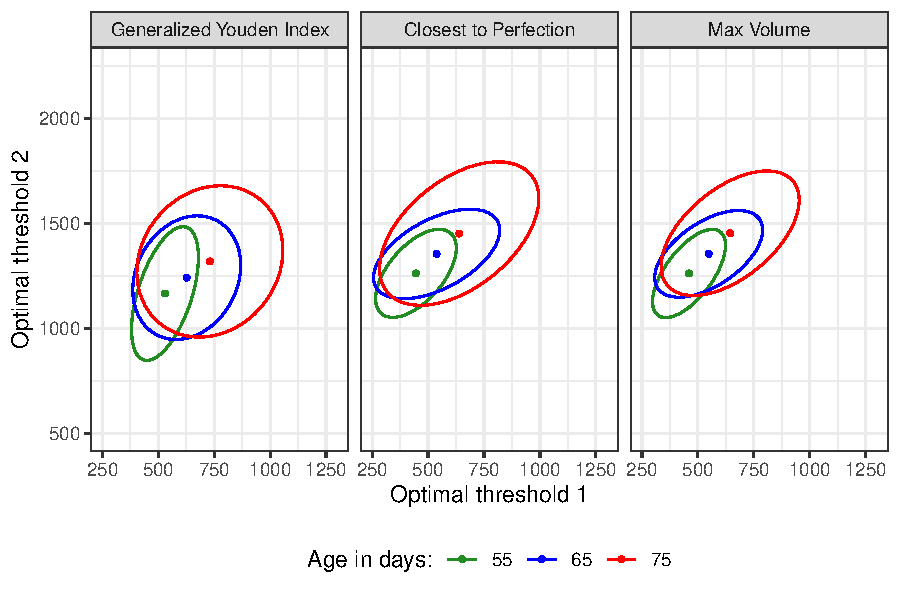
\includegraphics[width=0.8\textwidth]{optThres_ellip.pdf}
  \caption{The 95\% confidence regions for the age-specific optimal pairs of thresholds for three values of age: 55, 65, and 75.}
  \label{fig:optThresh}
\end{figure}


\hypertarget{house-cooking-fuel-choice}{%
\subsubsection{House cooking fuel
choice}\label{house-cooking-fuel-choice}}

We use the dataset \texttt{EnergyEthiopia} to illustrate the use of the package for evaluating a classifier in a three-class setting with panel data. The \texttt{EnergyEthiopia} data, included in the package, is a subset of the panel dataset discussed in \citet{alem2016modeling}. The full dataset is collected in 4 cities of Ethiopia (Addis Ababa, Awassa, Dessie and Mekelle) within three different years: 2000, 2004 and 2009. Each household participated in the study at most three times (three years). For each time, the information on household energy choice and some covariates such as expenditure, demographic indicators, household size and educational status, are recorded. \citet{alem2016modeling} used the full dataset to investigate the determinants of household fuel cooking choice and energy transition in urban Ethiopia, based on a random-effects multinomial logistic model.

The dataset, named \texttt{EnergyEthiopia}, includes 2088 observations from 1123 households living in Addis Ababa and the following variables:
\begin{itemize}
\item the cooking energy states of a household (\texttt{energy2}) with three categories: clean fuel only (denoted as 1), a mix of clean and biomass fuel (2) and biomass fuel only (1);
\item log real consumption per adult equivalent units (\texttt{lrconsaeu});
\item the household size (\texttt{hhs});
\item the log of firewood price (\texttt{lfirewood\_pr});
\item the log of charcoal price (\texttt{lcharcol\_pr});
\item the log of kerosene price (\texttt{lkerosene\_pr});
\item the log of electricity price (\texttt{lelectric\_pr}).
\end{itemize}

We are interested in evaluating the ability of the \emph{log real consumption per adult equivalent units} to discriminate three cooking energy states for a household, given the information provided by some covariates, such as the household size, the prices of firewood, charcoal and kerosene. Above, the term ``clean fuel only'' refers to clean energy sources such as electricity, gas and kerosene; whereas, ``biomass fuel only'' refers to energy sources such as firewood, charcoal, dung and crop residues. In our analysis, the 1123 households make up the clusters.


\begin{example}
> library(ClusROC)
> data("EnergyEthiopia")
\end{example}


As the first step, we fit a linear mixed-effects model for the response variable \texttt{lrconsaeu} with the covariates: \texttt{hhs\_ft}, \texttt{lfirewood\_pr}, \texttt{lcharcol\_pr} and \texttt{lkerosene\_pr}. Here \texttt{hhs\_ft} is a factor representing four levels of the household size: small (1 $\le$ \texttt{hhs} $\le$ 4), medium (5 $\le$ \texttt{hhs} $\le$ 8), large (9 $\le$ \texttt{hhs} $\le$ 12) and very large (\texttt{hhs} $\ge$ 13).
\begin{example}
> out_md_enery <- clus_lme(
+   fixed_formula = lrconsaeu ~ hhs_ft + lfirewood_pr + lcharcol_pr + lkerosene_pr,
+   name_class = "energy2", name_clust = "uqid",
+   data = EnergyEthiopia, boxcox = FALSE
+ )
The ordered levels of classes are specified by the order of 
 averages of the test values for each class:
3 < 2 < 1
\end{example}
As in the first application, we still have no information about the rank-ordered nature of the classifier (\texttt{lrconsaeu}) concerning the classes, so the monotone ordering was specified by ordering the classes according to the rank of the sample means of \texttt{lrconsaeu} inside the three groups. The results are shown as follows.
\begin{example}
> print(out_md_enery)

CALL: clus_lme(fixed_formula = lrconsaeu ~ hhs_ft + lfirewood_pr + 
    lcharcol_pr + lkerosene_pr, name_class = "energy2", name_clust = "uqid", 
    data = EnergyEthiopia, boxcox = FALSE)
 
Coefficients:
                              Est. Std.Error z-value  p-value    
energy23                   4.93925   0.11856  41.661  < 2e-16 ***
energy23:hhs_ftmedium     -0.48145   0.09126  -5.275 1.33e-07 ***
energy23:hhs_ftlarge      -0.77942   0.12139  -6.421 1.36e-10 ***
energy23:hhs_ftvery large -0.92139   0.14911  -6.179 6.44e-10 ***
energy23:lfirewood_pr     -0.09812   0.04806  -2.042  0.04119 *  
energy23:lcharcol_pr      -0.01146   0.08398  -0.136  0.89150    
energy23:lkerosene_pr     -0.13069   0.09731  -1.343  0.17927    
energy22                   5.14705   0.08235  62.502  < 2e-16 ***
energy22:hhs_ftmedium     -0.39801   0.06730  -5.914 3.33e-09 ***
energy22:hhs_ftlarge      -0.60084   0.09475  -6.341 2.28e-10 ***
energy22:hhs_ftvery large -0.63877   0.18434  -3.465  0.00053 ***
energy22:lfirewood_pr      0.02983   0.04203   0.710  0.47793    
energy22:lcharcol_pr      -0.10345   0.05570  -1.857  0.06329 .  
energy22:lkerosene_pr     -0.24888   0.08953  -2.780  0.00544 ** 
energy21                   5.05581   0.05928  85.283  < 2e-16 ***
energy21:hhs_ftmedium     -0.40857   0.04612  -8.859  < 2e-16 ***
energy21:hhs_ftlarge      -0.57306   0.06944  -8.252  < 2e-16 ***
energy21:hhs_ftvery large -0.74813   0.17193  -4.351 1.35e-05 ***
energy21:lfirewood_pr      0.05490   0.02776   1.978  0.04793 *  
energy21:lcharcol_pr      -0.11632   0.03957  -2.940  0.00328 ** 
energy21:lkerosene_pr      0.13104   0.06246   2.098  0.03590 *  
sigma_c                    0.47835   0.02062      --       --    
sigma_1                    0.55878   0.03409      --       --    
sigma_2                    0.49135   0.02568      --       --    
sigma_3                    0.57106   0.02103      --       --    
ICC                        0.43933        --      --       --    
---
Signif. codes:  0 ‘***’ 0.001 ‘**’ 0.01 ‘*’ 0.05 ‘.’ 0.1 ‘ ’ 1

Number of observations: 2088 
Number of clusters: 1123 
Sample size within cluster:
     Min      Max  Average 
1.000000 3.000000 1.859305 
Box-Cox transformation: FALSE
\end{example}
The diagnostic plots shown in Figure \ref{fig:diag-md-energy} seem to suggest that the normality assumption and the homogeneity of variances are reliable.
\begin{example}
> plot(out_md_enery)
\end{example}

\begin{figure}[htbp]
\centering
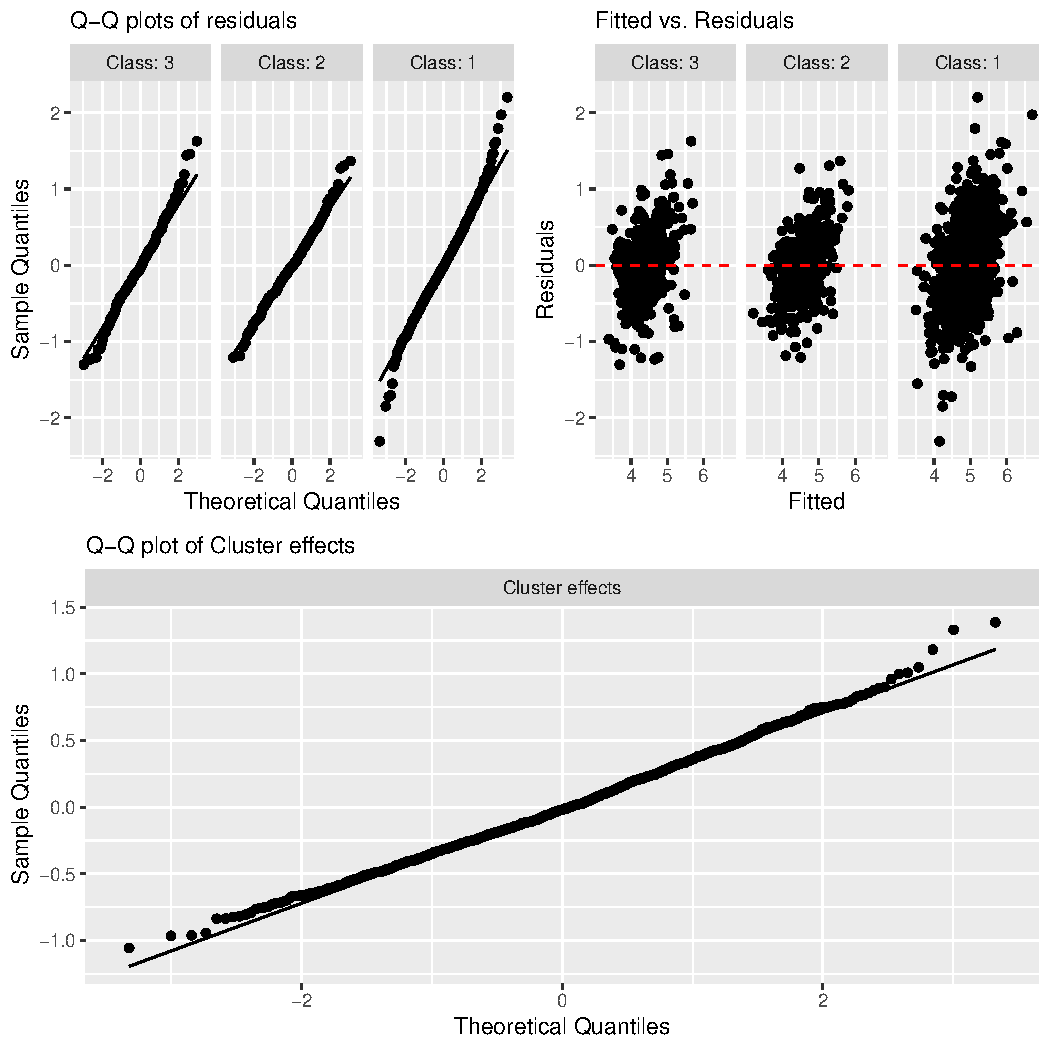
\includegraphics[width=0.7\linewidth]{diagnosis_model_energy.pdf} 
\caption{The diagnostic plots for the linear mixed-effects model (EnergyEthiopia data).}
\label{fig:diag-md-energy}
\end{figure}

We estimate the covariate-specific VUS at four different combinations of the covariates, when the value of \texttt{hhs\_ft} changes from ``small'' to ``very large'', the values of \texttt{lfirewood\_pr}, \texttt{lcharcol\_pr} and \texttt{lkerosene\_pr} are fixed as 1, $-1$ and 2, respectively. Here, the values ``1'' and ``2'' of \texttt{lfirewood\_pr} and \texttt{lkerosene\_pr} refer to the very high price of the firewood, and the kerosene, respectively, while the value ``-1'' of \texttt{lcharcol\_pr} refers to the very low price of the charcoal. The results of the covariate-specific VUS estimation procedure are displayed below.
\begin{example}
> out_vus_enery <- clus_vus(
+   out_clus_lme = out_md_enery,
+   newdata = data.frame(hhs_ft = c("small", "medium", "large", "very large"), 
+                        lfirewood_pr = c(1, 1, 1, 1), 
+                        lcharcol_pr = c(-1, -1, -1, -1), 
+                        lkerosene_pr = c(2, 2, 2, 2))
+ )
> print(out_vus_enery)

CALL: clus_vus(out_clus_lme = out_md_enery, newdata = data.frame(hhs_ft = c("small", 
    "medium", "large", "very large"), lfirewood_pr = c(1, 1, 
    1, 1), lcharcol_pr = c(-1, -1, -1, -1), lkerosene_pr = c(2, 
    2, 2, 2)))
 
Covariate-specific VUS: 
      Covariates Values  Est. Std.Error z-value p-value    
      (small, 1, -1, 2) 0.380    0.0674    3.17  <0.001 ***
     (medium, 1, -1, 2) 0.404    0.0639    3.72  <0.001 ***
      (large, 1, -1, 2) 0.443    0.0693    3.99  <0.001 ***
 (very large, 1, -1, 2) 0.440    0.0862    3.17  <0.001 ***
---
Signif. codes:    0 ‘***’ 0.001 ‘**’ 0.01 ‘*’ 0.05 ‘.’ 0.1 ‘ ’ 1
z-value and p-value are for testing the null hypothesis H0: VUS = 1/6 vs HA: VUS > 1/6
\end{example}
The estimated covariate-specific VUSs suggest that the accuracy of \texttt{lrconsaeu} increases as the household size increases while the other covariates are fixed. The inference results for covariate-specific VUS indicate that the \texttt{lrconsaeu} can be considered as a classifier for distinguishing a household using biomass fuel only from others using either clean fuel only or a mixed fuel. However, its accuracy is not so high. We also compute the 95\% confidence intervals for the covariate-specific VUS at four different points.
\begin{example}
> ci_clus_vus(out_vus_enery)

The 95\% confidence intervals for covariate-specific VUS:
   Covariates Values  Normal approximation  Logit transformation  Probit transformation
    (small, 1, -1, 2)       (0.248, 0.512)       (0.259, 0.518)         (0.257, 0.517)
   (medium, 1, -1, 2)       (0.279, 0.529)       (0.287, 0.533)         (0.286, 0.532)
    (large, 1, -1, 2)       (0.307, 0.579)       (0.314, 0.580)         (0.313, 0.580)
(very large, 1, -1, 2)      (0.271, 0.609)       (0.284, 0.609)         (0.281, 0.609)
\end{example}

Since the covariate point \texttt{("large", 1, -1, 2)} gives the highest covariate-specific VUS estimate among the considered points, we plot the covariate-specific ROC surface at this point, to visualize the covariate-specific TCFs at all possible pairs of thresholds. The result is displayed in Figure \ref{fig:ROC-surface-energy}.
\begin{example}
> clus_roc_surface(
+   out_clus_lme = out_md_enery,
+   newdata = data.frame(hhs_ft = "large", lfirewood_pr = 1,
+                        lcharcol_pr = -1, lkerosene_pr = 2),
+   file_name = "ROCS_Energy_ex1.png"
+ )
\end{example}

\begin{figure}[htbp]
\centering 
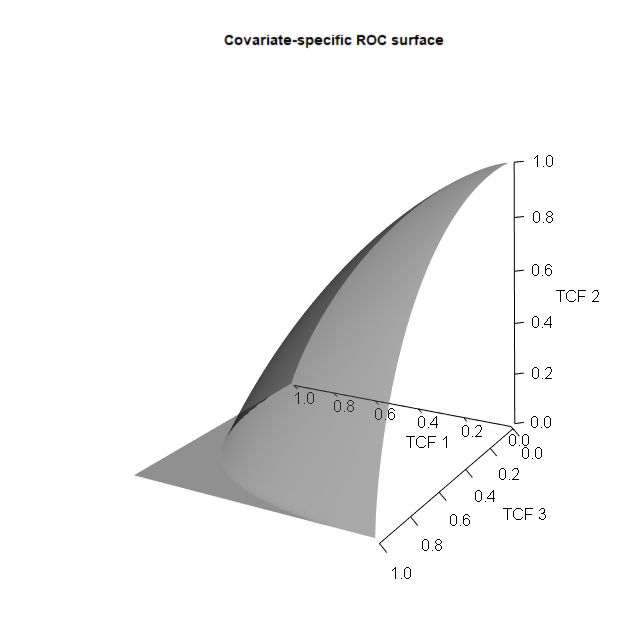
\includegraphics[width=0.5\linewidth]{ROCS_Energy_ex1} 
\caption{The plot of covariate-specific ROC surface at the covariate point \texttt{("large", 1, -1, 2)}.}
\label{fig:ROC-surface-energy}
\end{figure}

Now, suppose we consider a pair of thresholds as $(t_1, t_2) = (3.75, 4.75)$. The results of the estimation of the covariate-specific TCFs at that pair, associated with four different covariate points, are obtained by:
\begin{example}
> clus_tcfs(out_clus_lme = out_md_enery,
+           newdata = data.frame(
+             hhs_ft = c("small", "medium", "large", "very large"), 
+             lfirewood_pr = c(1, 1, 1, 1), lcharcol_pr = c(-1, -1, -1, -1), 
+             lkerosene_pr = c(2, 2, 2, 2)),
+           thresholds = c(3.75, 4.75), ap_var = TRUE)

CALL: clus_tcfs(out_clus_lme = out_md_enery, newdata = data.frame(hhs_ft = c("small", 
    "medium", "large", "very large"), lfirewood_pr = c(1, 1, 
    1, 1), lcharcol_pr = c(-1, -1, -1, -1), lkerosene_pr = c(2, 
    2, 2, 2)), thresholds = c(3.75, 4.75), ap_var = TRUE)
 
Covariate-specific TCFs at (3.75,4.75) : 
    Covariate(s) Values TCF 1 TCF 2 TCF 3 Se.TCF 1 Se.TCF 2 Se.TCF 3
      (small, 1, -1, 2) 0.126 0.415 0.839   0.0569   0.0617   0.0366
     (medium, 1, -1, 2) 0.312 0.526 0.671   0.0906   0.0247   0.0532
      (large, 1, -1, 2) 0.467 0.532 0.588   0.1100   0.0147   0.0612
 (very large, 1, -1, 2) 0.543 0.529 0.495   0.1230   0.0247   0.1080
\end{example}

Finally, we obtain the covariate-specific optimal pairs of thresholds at four different covariate points, based on all criteria, i.e., GYI, CtP and MV.
\begin{example}
> out_thresh_enery <- clus_opt_thres3(
+   method = c("GYI", "CtP", "MV"), out_clus_lme = out_md_enery,
+   newdata = data.frame(hhs_ft = c("small", "medium", "large", "very large"), 
+                        lfirewood_pr = c(1, 1, 1, 1), 
+                        lcharcol_pr = c(-1, -1, -1, -1), 
+                        lkerosene_pr = c(2, 2, 2, 2)),
+   ap_var = TRUE
+ )
> print(out_thresh_enery)

CALL: clus_opt_thres3(method = c("GYI", "CtP", "MV"), out_clus_lme = out_md_enery, 
    newdata = data.frame(hhs_ft = c("small", "medium", "large", 
        "very large"), lfirewood_pr = c(1, 1, 1, 1), lcharcol_pr = c(-1, 
        -1, -1, -1), lkerosene_pr = c(2, 2, 2, 2)), ap_var = TRUE)
 
Covariate-specific optimal pair of thresholds: 
    Covariate(s) Values                   Method Threshold 1 Threshold 2 TCF 1 TCF 2 TCF 3
      (small, 1, -1, 2) Generalized Youden Index        4.52        5.18 0.460 0.370 0.661
      (small, 1, -1, 2)    Closest to Perfection        4.51        5.35 0.455 0.453 0.572
      (small, 1, -1, 2)               Max Volume        4.51        5.35 0.454 0.452 0.575
     (medium, 1, -1, 2) Generalized Youden Index        4.13        4.78 0.509 0.363 0.657
     (medium, 1, -1, 2)    Closest to Perfection        4.08        4.94 0.481 0.465 0.574
     (medium, 1, -1, 2)               Max Volume        4.07        4.93 0.480 0.464 0.578
      (large, 1, -1, 2) Generalized Youden Index        3.91        4.59 0.553 0.379 0.669
      (large, 1, -1, 2)    Closest to Perfection        3.84        4.74 0.514 0.486 0.591
      (large, 1, -1, 2)               Max Volume        3.83        4.73 0.512 0.483 0.597
 (very large, 1, -1, 2) Generalized Youden Index        3.84        4.50 0.592 0.369 0.627
 (very large, 1, -1, 2)    Closest to Perfection        3.74        4.63 0.535 0.485 0.560
 (very large, 1, -1, 2)               Max Volume        3.74        4.63 0.535 0.483 0.562

Standard errors of Covariate-specific optimal pair of thresholds: 
    Covariate(s) Values                   Method SE. Threshold 1 SE. Threshold 2
      (small, 1, -1, 2) Generalized Youden Index           0.234          0.1040
      (small, 1, -1, 2)    Closest to Perfection           0.112          0.0914
      (small, 1, -1, 2)               Max Volume           0.114          0.0932
     (medium, 1, -1, 2) Generalized Youden Index           0.166          0.0990
     (medium, 1, -1, 2)    Closest to Perfection           0.110          0.0868
     (medium, 1, -1, 2)               Max Volume           0.111          0.0891
      (large, 1, -1, 2) Generalized Youden Index           0.158          0.1090
      (large, 1, -1, 2)    Closest to Perfection           0.122          0.0954
      (large, 1, -1, 2)               Max Volume           0.123          0.0988
 (very large, 1, -1, 2) Generalized Youden Index           0.192          0.1640
 (very large, 1, -1, 2)    Closest to Perfection           0.154          0.1390
 (very large, 1, -1, 2)               Max Volume           0.154          0.1410
\end{example}
The 95% confidence regions for the covariate-specific optimal pairs of thresholds are shown in Figure \ref{fig:optThresh-energy}.
\begin{example}
> plot(out_thresh_enery, colors = c("orange", "red", "blue", "forestgreen"), 
+      file_name = "optThres_energy_ellip.pdf", nrow_legend = 2, 
+      width = 6, height = 4)
\end{example}

\begin{figure}[htbp]
\centering
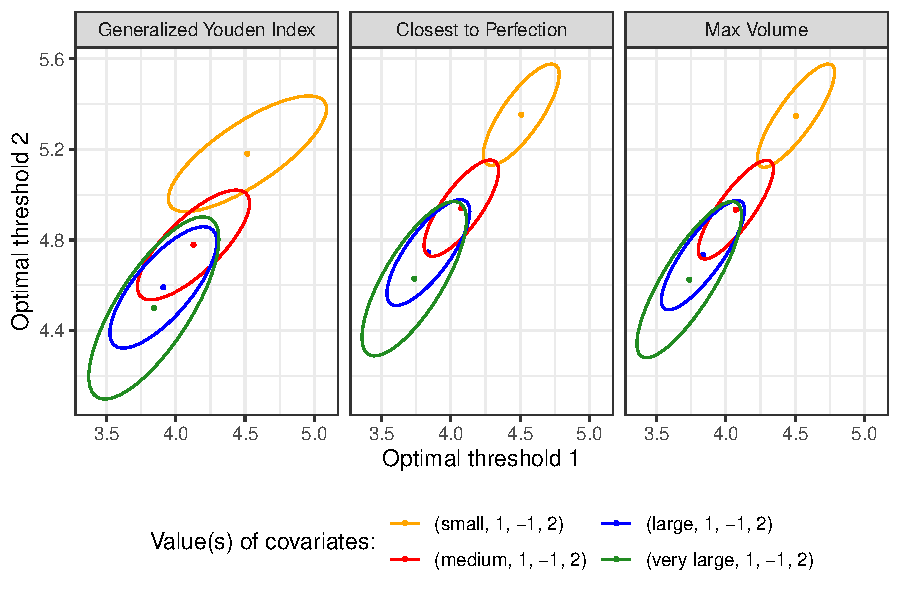
\includegraphics[width=0.8\linewidth]{optThres_energy_ellip.pdf} 
\caption{The 95\% confidence regions for the age-specific optimal pairs of thresholds for four covariate points (in the house cooking fuel choice example).}
\label{fig:optThresh-energy}
\end{figure}


\hypertarget{conclusion}{%
\section{Conclusion}\label{conclusion}}
This paper introduces the \pkg{ClusROC} package, the first R package for ROC surface analysis in three-class classification problems, for clustered data and in the presence of covariates. The package allows obtaining point estimates and confidence regions for true class fractions, ROC surface estimates and plots, point and interval estimates of VUS, and point estimates and confidence regions for optimal pair of thresholds. In the last case, three different criteria can be used: GYI, CtP, and MV. The package is available on Comprehensive R Archive Network (CRAN) at \url{http://CRAN.R-project.org/package=ClusROC}. The functions in the package are described and implemented using, as examples, the real datasets \texttt{MouseNeurons} and \texttt{EnergyEthiopia} provided in the package itself. 

The linear mixed-effects model relies on the assumptions of normality and homoscedasticity. When such assumptions do not hold, the Box-Cox transformation can be employed.  In these cases, a bootstrap procedure is needed to estimate the elliptical confidence regions for the optimal thresholds. This procedure can take a long computation time depending on the size of the data (either the number of clusters or the sample size within the clusters). For this reason, we recommend users enable the parallel computation option, which is already implemented within the function \texttt{clus\_opt\_thres3()}.


\hypertarget{acknowledgments}{%
\section{Acknowledgments}\label{acknowledgments}}
This research was supported by the Ministero dell'Istruzione, dell'Università e della Ricerca-Italy (grant number DIFO\_ECCELLENZA18\_01). The authors acknowledge the Editor and two anonymous reviewers whose valuable suggestions contributed to improving the presentation of the contents.

\bibliography{refs_ClusROC.bib}

%%% Appendix - result of model for MouseNeurons without Box-Cox transformation
\hypertarget{appendix}{%
\section{Appendix}\label{appendix}}

To help the reader evaluate the need for transforming the data, we report here the results of the analysis based on the linear mixed-effects model without the Box-Cox transformation. The results show that the assumptions of normality and homoscedasticity are violated.

\begin{example}
> out_md_0 <- clus_lme(fixed_formula = Lamp5_cpm ~ age_days,
+                      name_class = "subclass_label", name_clust = "genotype_id",
+                      data = MouseNeurons)
The ordered levels of classes are specified by the order of 
 averages of the test values for each class:
L4 < L5 PT < L2/3 IT  
\end{example}

\begin{example}
> print(out_md_0)

CALL: clus_lme(fixed_formula = Lamp5_cpm ~ age_days, name_class = "subclass_label", 
    name_clust = "genotype_id", data = MouseNeurons)
 
Coefficients:
                                    Est. Std.Error z-value  p-value    
subclass_labelL4               -378.9740  208.6613  -1.816   0.0693 .  
subclass_labelL4:age_days        11.3966    1.4166   8.045 8.62e-16 ***
subclass_labelL5 PT             558.0245   89.6372   6.225 4.80e-10 ***
subclass_labelL5 PT:age_days      8.6915    0.6581  13.207  < 2e-16 ***
subclass_labelL2/3 IT          1227.4463  251.7121   4.876 1.08e-06 ***
subclass_labelL2/3 IT:age_days    5.0032    3.4950   1.432   0.1523    
sigma_c                         330.1655   68.9777      --       --    
sigma_1                         529.2924    9.1052      --       --    
sigma_2                         514.0238   12.5033      --       --    
sigma_3                         611.5288   30.7857      --       --    
ICC                               0.2638        --      --       --    
---
Signif. codes:  0 ‘***’ 0.001 ‘**’ 0.01 ‘*’ 0.05 ‘.’ 0.1 ‘ ’ 1

Number of observations: 860 
Number of clusters: 23 
Sample size within cluster:
     Min      Max  Average 
  1.0000 330.0000  37.3913 
Box-Cox transformation: FALSE 
\end{example}

\begin{example}
> plot(out_md_0)
\end{example}

\begin{figure}[htbp]
\centering 
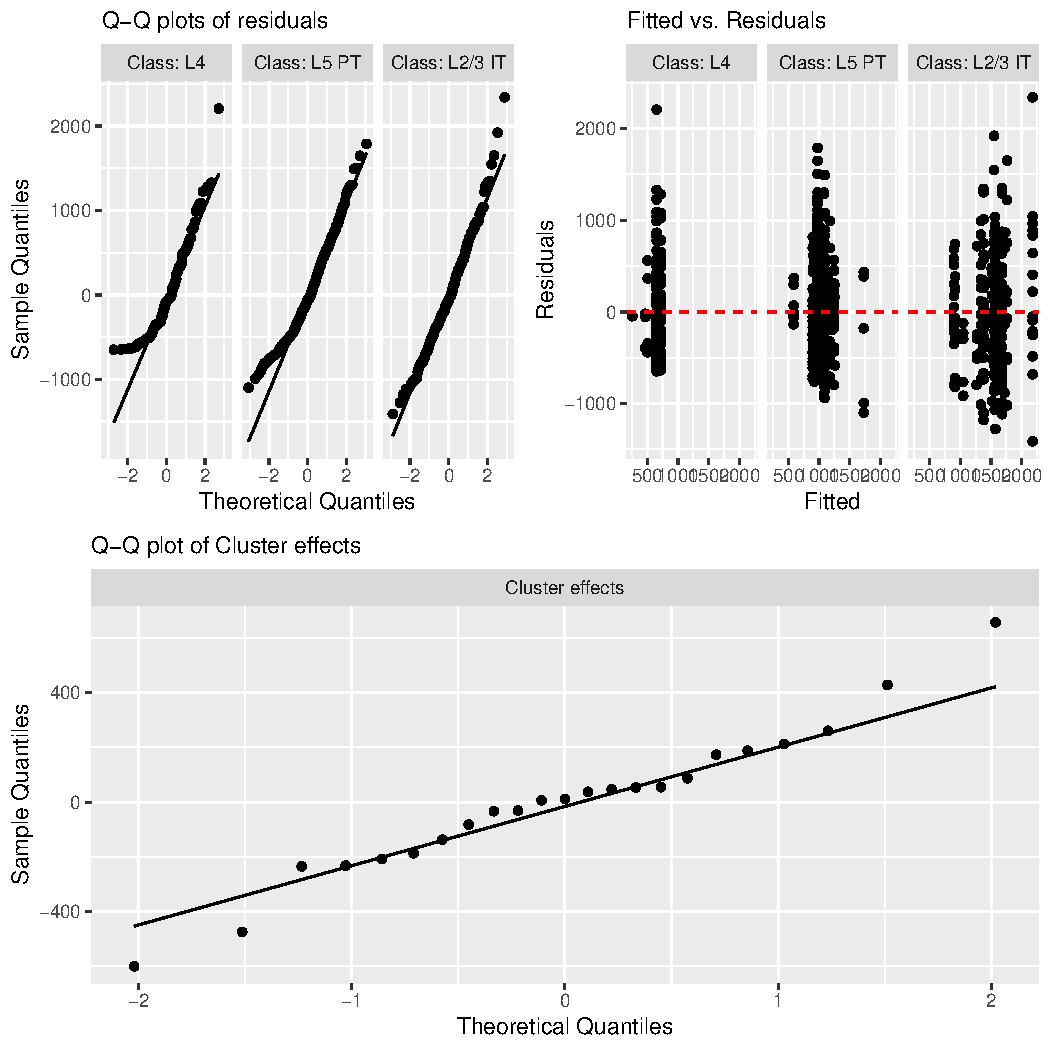
\includegraphics[width=0.7\linewidth]{diagnosis_model_0.pdf}
\caption{The diagnostic plots for the linear mixed-effects model for \texttt{MouseNeurons} data, without Box-Cox transformation.}
\label{fig:diag-md-0}
\end{figure}

%%%
\address{%
Duc-Khanh To\\
University of Padova\\%
Department of Statistical Sciences\\ Via C. Battisti, 241; I-35121
Padova, Italy\\
and \\
Department of Information and Engineering \\
Via Gradenigo, 6/b; 35131 Padova, Italy\\
%
%
\textit{ORCiD: \href{https://orcid.org/0000-0002-4641-0764}{0000-0002-4641-0764}}\\%
\href{mailto:duckhanh.to@unipd.it}{\nolinkurl{duckhanh.to@unipd.it}}%
}

\address{%
Gianfranco Adimari\\
University of Padova\\%
Department of Statistical Sciences\\ Via C. Battisti, 241; I-35121
Padova, Italy\\
%
%
\textit{ORCiD: \href{https://orcid.org/0000-0002-7811-912X}{0000-0002-7811-912X}}\\%
\href{mailto:gianfranco.adimari@unipd.it}{\nolinkurl{gianfranco.adimari@unipd.it}}%
}

\address{%
Monica Chiogna\\
University of Bologna\\%
Department of Statistical Sciences ``Paolo Fortunati'\,'\\ Via Belle
Arti, 41; 40126 Bologna, Italy\\
%
%
\textit{ORCiD: \href{https://orcid.org/0000-0002-7238-3739}{0000-0002-7238-3739}}\\%
\href{mailto:monica.chiogna2@unibo.it}{\nolinkurl{monica.chiogna2@unibo.it}}%
}
